\documentclass[dvipsnames,format=sigconf,anonymous=False,review=false, balance=false]{acmart}


\AtBeginDocument{%
  \providecommand\BibTeX{{%
    \normalfont B\kern-0.5em{\scshape i\kern-0.25em b}\kern-0.8em\TeX}}}

\setcopyright{acmcopyright}
\copyrightyear{2023}
\acmYear{2023}
\acmDOI{XXXXXXX.XXXXXXX}

\acmConference[GECCO'23]{Genetic and Evolutionary Computation Conference}{July 15-19,
  2023}{Lisbon, Portugal}
\acmBooktitle{GECCO '23: ACM Genetic and Evolutionary Computation Conference,
    July 15-19, 2023, Lisbon, Portugal} 
\acmPrice{15.00}
\acmISBN{978-1-4503-XXXX-X/18/06}

\newcommand{\ct}[1]{\textit{\textcolor{purple}{(#1)}}}
\newcommand{\ma}[1]{\textit{\textcolor{blue}{(#1)}}}
\newcommand{\fr}[1]{\textit{\textcolor{red}{(#1)}}}

\usepackage{enumitem}
\usepackage{arydshln}

\begin{document}

\title{Socialz: Multi-Feature Social Fuzz Testing}

\author{Francisco Zanartu}
\affiliation{%
  \institution{The University of Adelaide}
  \city{Adelaide}
  \country{Auustralia}}
\email{francisco.zanartu@adelaide.edu.au}

\author{Christoph Treude}
\affiliation{%
  \institution{The University of Melbourne}
  \city{Melbourne}
  \country{Australia}}
\email{christoph.treude@unimelb.edu.au}

\author{Markus Wagner}
\affiliation{%
  \institution{Monash University}
  \city{Clayton}
  \country{Australia}}
\email{markus.wagner@monash.edu}



\begin{abstract}

Online social networks have become an integral aspect of our daily lives and play a crucial role in shaping our relationships with others. However, bugs and glitches, even minor ones, can cause anything from frustrating problems to serious data leaks that can have far-reaching impacts on millions of users.

To mitigate these risks, fuzz testing, a method of testing with randomised inputs, can provide increased confidence in the correct functioning of a social network. However, implementing traditional fuzz testing methods can be prohibitively difficult or impractical for programmers outside of the network's development team. 

To tackle this challenge, we present Socialz, a novel approach to social fuzz testing that 
(1) characterises real users of a social network, 
(2) diversifies their interaction using evolutionary computation across multiple, non-trivial features, and 
(3) collects performance data as these interactions are executed. 
With Socialz, we aim to provide anyone with the capability to perform comprehensive social testing, thereby improving the reliability and security of online social networks used around the world.

\end{abstract}

\keywords{Fuzz testing; graph social network; diversity optimisation.}

\maketitle

\sloppy

\section{Introduction}
Online social networks (OSNs) are an integral part of modern society, influencing a wide range of aspects of our daily lives. The vast quantity of personal information shared on these platforms makes them a treasure trove for companies seeking to reach out to potential customers and for individuals looking to grow their social circle or entertain themselves. However, like any software, OSNs are prone to bugs and technical issues; consequences range from poor user experience~\cite{brodkin2022socialapp,day2015socialbugs} to massive data breaches affecting billions of individuals~\cite{morahan2022dataleaks}.

The recent rise of social bugs in software systems has prompted the need for social testing~\cite{ahlgren2020wes}. However, for the research community, social testing poses several challenges. 
First and foremost, obtaining data from online social networks (OSNs) can be time-consuming, resource-intensive, and requires specialised expertise, which may not be accessible to non-specialists~\cite{https://doi.org/10.48550/arxiv.1612.04666}. For example, privacy policies and community guidelines may restrict access to data, making it unavailable to researchers; Furthermore, descriptions of data extraction methods are often omitted in many studies~\cite{info:doi/10.2196/13544}. 
Second, researchers may be limited in their ability to conduct experiments on OSN systems if they are built using proprietary software platforms~\cite{ahlgren2020wes}. 
Finally, the sheer size and complexity of OSN systems can result in significant operational costs, which can impede researchers' ability to conduct large-scale experiments, limiting the scope and depth of their research.

To overcome these challenges, technology companies develop tools such as Web-Enabled Simulation (WES, by Facebook/Meta)~\cite{ahlgren2020wes}, allow developers to test code updates and new features in a simulated environment, without risking real user data. 
Social testing, which involves simulating interactions among a large community of users, can be used to uncover faults in online social networks. 
However, these tools are not widely available to the public and may have limitations in simulating the full spectrum of user behaviours that could result in uncovering bugs. 



To address these limitations, we introduce Socialz, an approach for social fuzz testing, which makes the following key contributions: 

\setlist[itemize]{leftmargin=7mm}
\setlist[enumerate]{leftmargin=8.5mm}

\begin{enumerate}
    \item characterisation of users of a real social network, 
    \item evolutionary diversification of community interaction with respect to multiple, non-trivial features, 
and 
    \item a workflow for executing interactions in the system and collecting performance data.
\end{enumerate}

Socialz aims to advance the field of social testing through diversity-based user behaviour. Our approach involves evolving diverse sets of virtual users that are diversified and unbiased across a non-trivial feature space. This allows us to cover a wider range of behaviours compared to real users, and increases the likelihood of uncovering bugs that may not be detected by a set of similar and biased virtual users. 


\section{Related Work}

Software testing has evolved into a vast field that includes many different methods and techniques for assessing the performance, usability, and other attributes of software systems~\cite{7814898}. Testing is performed at various levels of abstraction, ranging from unit testing to system testing.


Recently, the concept of social testing has emerged as a new level of abstraction, potentially positioned above system testing~\cite{ahlgren2020wes}. This is due to the recognition that social bugs can arise through community interactions and may not be uncovered by traditional testing that focuses solely on single user journeys~\cite{harman2018journeys}. 

In the following overview, we will briefly examine prior work in the testing of social networks, the application of evolutionary methods in fuzz testing, and diversity optimisation.

\subsection{Testing of Social Networks}

Search-Based Software Testing (SBST) is a technique that leverages optimization search algorithms to solve software testing problems~\cite{5954405}. This approach is widely used in both industrial and academic sectors, including at Facebook, where it is employed to test the behaviour of both the system and its users~\cite{10.1007/978-3-319-99241-9_1}.

In social networks, testing goes beyond simply assessing the behaviour of the system and involves evaluating the interactions between users facilitated by the platform. To that end, Web-Enabled Simulation (WES) simulates the behaviours of a community of users on a software platform using a set of bots~\cite{ahlgren2020wes}. Traditional tests, on the other hand, involve executing a predetermined series of input steps. WES is run in-vivo but in a shadow copy of the system, hence as a separate ``digital twin'', which allows for testing without risk to real user data~\cite{ahlgren2021facebook}. Both ``digital twins'' and WES have widespread industrial applications, not only in OSNs but also in robotics, manufacturing, healthcare, transport, and the energy sector, among others~\cite{jiang2021industrial,8972429}.

In addition to testing, there are also methods for formally verifying the correctness of social network software and systems. Formal verification of social network protocols and algorithms ensures security and reliability by ensuring access to content is subject to both user-specified and system-specified policies~\cite{cheng2012user,kafali2014detecting}. Model checking can be applied at various levels of abstraction, from high-level network properties to the implementation of individual components~\cite{pardo2017model}. This approach can be used in combination with other testing techniques, such as simulation or testing with software-controlled bots, to provide a more comprehensive evaluation of a social network's behaviour and performance~\cite{pedersen2021social}.


\subsection{Evolutionary Fuzzing}

We adopt definitions from~\citet{https://doi.org/10.48550/arxiv.1812.00140}, who define fuzzing as a software testing methodology  that involves injecting unexpected or randomised input data into a program under test (PUT) to uncover defects or bugs. A specific application of fuzzing, called fuzz testing, evaluates the security policy violations of the PUT. The tool used to perform fuzz testing is known as a fuzzer.

he inputs used in fuzzing can be selected either randomly, with each element having an equal chance of being chosen, or through guided methods such as syntactic or semantic models~\cite{MARIANI2015bbtesting}. 
Evolutionary fuzz testing is a variant of fuzz testing that leverages evolutionary algorithms to optimise the input data. Research has shown that it is effective in discovering a wide range of vulnerabilities, including those that are difficult to detect with traditional testing methods. For example, \citet{li2019v} demonstrate V-Fuzz, a vulnerability-oriented evolutionary fuzzing framework that combines vulnerability prediction with evolutionary fuzzing to 
reach potentially vulnerable code. They test various open-source Linux applications and fuzzing benchmarks. 
For Android applications, \citet{Cotroneo_2019} introduce a coverage-guided fuzzing platform that demonstrated to be more efficient than blind fuzzing. 
Similarly, \citet{9847081} employ a constrained neural network evolutionary search method to optimise the testing process and efficiently search for traffic violations.

Although fuzzing is widely used, to the best of our knowledge, no research has been conducted to fuzz test a social network system. 

\subsection{Diversity Optimisation}\label{sec:diversityopt}

When it comes to social fuzz testing, the actions a user takes need to be determined, such as ``follow a particular person''. In such a case, defining a user that achieves exactly this goal is straightforward, as a developer can easily translate the desired outcome into a specific interaction. 
However, creating a user with a more complex behaviour, such as ``a virtual user should be highly active but not very central to everything that is going on'', is not as simple. Mapping the desired interaction between the virtual user and its environment is challenging due to the intricate interplay, even though the activity and centrality calculations may not be black boxes by definition. 
This issue becomes even more complex when designing a group of virtual users within a social network that can interact with each other in various ways.

We propose a practical solution to addressing such issues by treating the functions as black boxes and utilising heuristic approaches like novelty search~\cite{DBLP:conf/gecco/RisiVHS09} or evolutionary diversity optimisation~\cite{DBLP:conf/gecco/UlrichT11}. 

This is made possible by recent algorithmic advancements in diversity optimisation with multiple features. 
First, the discrepancy-based approach by \citet{neumann2018discrepancy} aims to minimise the discrepancy of the solution set in the feature space. The discrepancy measure is effectively an indicator function that assesses the set of given solutions in the feature space.
Second, \citet{neumann2019moo} present approaches based on space transformations and multi-objective performance indicators. Among other, these formulations are used to create (1) sets of images (with 149x149 pixels) 
that are diverse with respect to aesthetic or general features and (2) sets of instances for the travelling salesperson problem 
(with up to 2000 cities) 
that are diverse with respect to features like hull ratio and minimum spanning tree depth~\cite{bossek2019tsplarge}.


\section{The Methodology of Socialz: Overview}\label{sec:methodology}

In the following, we present our three-stage approach for fuzz testing OSNs. Each of the following three sections is dedicated to one of the stages, and each of them has a distinct methodology.

In \textit{Stage 1/3: Characterisation of User Behaviour}, we detail the process of obtaining and analysing data from a real OSNs to understand the behaviour of users on the network. 
\textit{Stage 2/3: Evolutionary Diversification of Community Interaction} employs evolutionary algorithms to improve the diversity of user behaviour in the network, and 
\textit{Stage 3/3: Execution} involves  evaluating the evolved network. 

\paragraph{Target platform.} \label{sec:gitlab} 
To demonstrate Socialz, we need to choose a server as the PUT. The server needs to  meet certain requirements to ensure that the case study can be conducted: 

\begin{itemize}
\item A freely available, open-source server that can be self-hosted.
\item An API connection or similar to impersonate users on a network and to simulate events being created by them, necessary for accurately modelling the behaviour of users in a network.
\item The ability to gather system performance data.
\item The option to easily restart the system in order to achieve comparable conditions for the eventual evaluation.
\item A well-documented application for easy troubleshooting of problems that may arise during installation, maintenance, and operation of the system.
\end{itemize}

GitLab Community Edition (GitLab~CE) is the best fit for these requirements. 
GitLab~CE is the free and open source edition of GitLab, which is a platform that has over 30 million registered users~\cite{gitlabusers}. 
Despite being free, GitLab~CE provides a comprehensive set of performance metrics that are continually stored on an internal Prometheus time-series database. This database can be scrapped with a comprehensive set of pre-defined Grafana dashboards~\cite{gitlabdocumentation}, providing a wide range of performance metrics for our purposes (see Figure~\ref{fig:grafana} for an example).

\begin{figure}
\centering
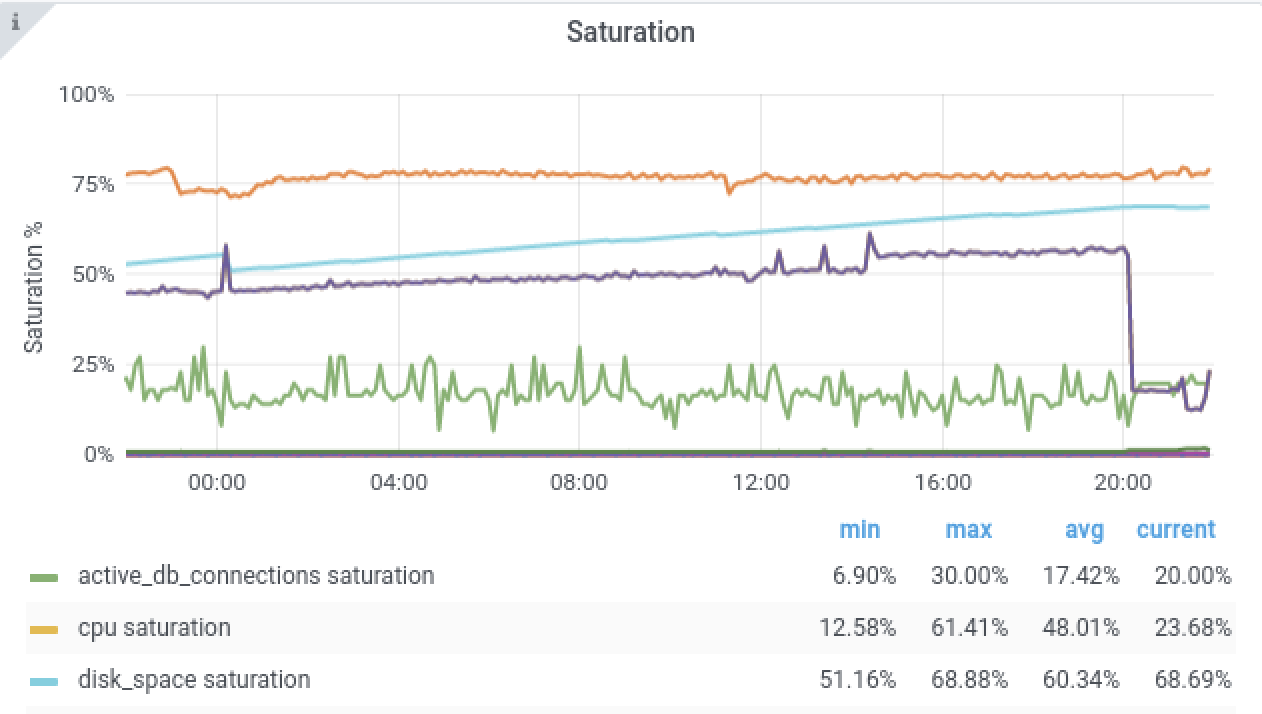
\includegraphics[width=\linewidth,trim=0 0 0 0,clip]{grafana.png}\vspace{-1mm}
\caption{Example of a Grafana dashboard, showing statistics of our running GitLab~CE server.}
\label{fig:grafana}
\end{figure}

To easily reset the system to well-defined states, we run GitLab~CE 15.5 in a Docker container, allowing us to delete the data and to restart the container to achieve a reproducible, initial state. Our system runs on a Ubuntu 22.04 virtual machine with 4 CPU cores, 100 GB of hard drive disk space, and 8 GB of RAM. 

\section{Characterisation of User Behaviour (Stage 1/3)}

As the starting point for this project, we populate our GitLab server with real-world data from GitHub. We use GitHub as our data source because it offers the largest repository of information with the kind of data that our platform needs and because it has a large community of over 100 million developers~\cite{dohmke2023million}, as well as comprehensive documentation that makes it easy to get started, troubleshoot issues, and find help. There are also several Git server alternatives, such as Gitea and Gogs\footnote{\url{https://gitea.io}, \url{https://gogs.io}. Retrieved 25 January 2023.}, that can be self-hosted and have similar features (but not the server performance metrics that GitLab offers), making it easy to transfer solutions from GitHub to them in terms of data. Additionally, projects exist that provide access to user interaction data that is similar to that found in online social networks (OSNs). These interactions include creating and annotating content, creating networks (e.g. starring a repository, linking comments), as well as ``malicious'' interactions (e.g. intentionally or unintentionally submitting bugs, spamming, or violating privacy). One such project that provide datas on interactions is GH~Archive\footnote{\url{https://www.gharchive.org}.  Retrieved 25 January 2023.}. It is a public dataset available on Google Big Query that has been recording the public GitHub timeline since 2011, and it makes this data easily accessible through SQL-like queries of JSON-encoded events as reported by the GitHub API.

To narrow down the immense amount of data available in GH~Archive\footnote{As of December 2022, the GH~Archive data stored on Google BigQuery totals more than 17.23 terabytes.}, we choose a sub-community within GitHub, and after considering various sub-communities based on their size, we find that COBOL's is small enough to enable us to conduct a thorough analysis of the data. This is an intentional choice, because we target a ``complete'' subset of the data, i.e. not a random sample of nodes or edges from GH~Archive that are not interconnected. We model the data as a graph, with users and repositories as nodes and GitHub events as edges. In this model, repositories can be thought of as groups on an online social network (OSN) where users share and contribute content. 

To focus on content creation, content annotation, and network creation, we select the following fives types of GitHub events:
\begin{itemize}
\item WatchEvents and ForkEvents can be likened to liking a public profile page.
\item PushEvents can be thought of as being invited to a group with permission to publish some content.
\item PullRequests can be thought of as requesting permission to publish something to a group.
\item FollowEvents represent establishing a connection or friendship with another user. Unfortunately, as of December 2013 FollowEvents have stopped being recorded in GH~Archive, we need to create a workaround where connections between users are based on their similarity. To ensure consistency in our analysis, we disregard the existing FollowEvents in the GH~Archive data and instead utilise only our own approach (see Section~\ref{sec:solrep}).
\end{itemize}

Finally, to ensure that our dataset is as complete as possible, we further adjust its size by filtering it to only include events from the years 2011 to 2016. This decision allows us to compile a relatively complete dataset (i.e. starting from the beginning of GH~Archive's records and going up to a particular date), rather than having more recent but incomplete data (e.g. like considering the last six years until today) in which possibly all relevant events would have occurred before the starting date of the snapshot. 

Table~\ref{tab:original} summarises the events in the original dataset, which we represent internally as an edge list containing 6,742 events between users and repositories.

\begin{table}
\centering
\caption{Original dataset: 1,523 users created a total of 6,742 events involving 156 repositories and forks (2011--2016).}
\label{tab:original}\vspace{-1mm}
\begin{tabular}{cc}
  \toprule
  \textbf{Event type} & \textbf{Number of events} \\
  \midrule
  PushEvent & 4234 \\
  WatchEvent & 1206 \\
  PullRequestEvent & 852 \\
  ForkEvent & 450 \\
  \bottomrule
\end{tabular}
\end{table}

\section{Evolutionary Diversification of Community Interaction (Stage 2/3)}

In this section, we outline the components of our evolutionary approach and how they are used to diversify a set of virtual users, which are less biased than their real-world counterparts. This process has the potential to reveal anomalies or unexpected behaviours that would otherwise be difficult to detect in sets of bots that are similar and biased.

\subsection{Features of Community Interaction}

To characterise users, we investigate three features that we consider to be non-trivial in the sense introduced in Section~\ref{sec:diversityopt}: given these features, a developer may struggle to manually design a set of virtual users that exhibit a spread of desired community interactions. 
Our chosen features allow us to characterise how active a user is, what is its relative importance and with what kind of events occur: 
\begin{itemize}
\item The graph degree of centrality measure of the nodes quantifies how active a user is in the network, i.e. how many events are submitted. This measure is often used as a notion of popularity in social networks~\cite{https://doi.org/10.48550/arxiv.2011.01627}, as nodes with a large number of relationships are considered more powerful and central, but has a limitation in that it only takes into account local knowledge of the network topology. Hence, we introduce an additional centrality metric to supplement its analysis next. 
\item To assess the relative importance of a particular user on the network, we utilise the PageRank algorithm~\cite{page1999pagerank}: it is fast to compute, well suited for a directed network such as ours and has been proven to be effective in characterising users~\cite{9420317}.
\item To characterise the types of actions a user performs --- for example, a user may submit only PushEvents, or only ForkEvents and PullRequestsEvents --- we represent each of the 15 possible combinations as a binary vector and then considered the corresponding decimal value as that user's ``event type''.\footnote{Because the number of users is much larger than the number of possible combinations, and because we aim for diversity, we conjecture that variations to this mapping procedure only have minor effects on the overall outcomes.} We consider 15 combinations, as we have four event types that are not FollowEvents, and the combination of ``user does not interact at all'' is not allowed.
\end{itemize}

It is critical to emphasise that these three metrics are features, not objectives: no user is ``better'' or ``worse'' than another one, neither in a single-objective sense, nor in a multi-objective sense.

\subsection{Solution Evaluation}\label{sec:solrep}

In our evolutionary setup, each individual is an interaction graph that represents how virtual users interact in a social network. 
In particular, each individual is an edge list that contains all the necessary information of our graph: the source node, the target node, and the type of event. 

\begin{table}
\caption{Original dataset: matrix representation. 
Users 658 and 659 are chosen to show non-zero data, as the matrix is sparsely populated.}
\label{tab:solutionrep}\vspace{-3mm}\setlength{\tabcolsep}{0.5mm}
\centering
\begin{tabular}{c|ccc:cccccc|}
      & repo$_1$ & $\cdots$ & \multicolumn{1}{c}{repo$_{156}$} & user$_1$ & $\cdots$ & user$_{658}$ & user$_{659}$ & $\cdots$ &   \multicolumn{1}{c}{user$_{1523}$} \\ \hline
repo$_1$ & 0         &     & 0     & 0    & & 0&4     &     & 0     \\
$\vdots$   &           &     &       &       &  &  &    &     &       \\
repo$_{156}$ & 0        &     & 0     & 0   &  & 0 & 0    &     & 0     \\ \cdashline{2-10}
user$_1$ & 0        &     & 0     & 0    & & 1 & 0    &     & 0     \\
$\vdots$ &&&&&&&&&\\
user$_{658}$ & 0        &     & 0     & 1    & & 0 &0     &     & 0     \\
user$_{659}$ & 4        &     & 0     & 0    & & 0 & 0 &        & 0     \\
$\vdots$   &    &       &     &       &       &       &  &    &       \\ 
user$_{1523}$     & 0     &     & 0     & 0   &  & 0 & 0    &     & 0 \\ \cline{2-10}
\end{tabular}
\end{table}

To evaluate our graphs, we have defined the following steps:
\begin{enumerate}
\item We first transform the edge list into an two-dimensional adjacency matrix. This adjacency matrix has four areas that reflect the interactions repo-repo, repo-user, user-repo, and user-user (see Table~\ref{tab:solutionrep}). 
\item We record the interactions between users and repositories in the repo-user and user-repo areas by summing the number of events that occur between each repository and user. Each event has a weight of one, regardless of its type. 
At present, as we do not further differentiate, the repo-user and the user-repo areas are mirrored versions of each other. 
\item As there are no interactions between repositories in our approach, the repo-repo area is always filled with zeros.
\item We use the user-user area to store FollowEvents. It is initially empty, and we fill it with data by evaluating the cosine similarity of the users based on their interactions with repositories (areas user-repo, repo-user). 
If the cosine similarity is greater than zero for a pair of two users, then we set the respective entry to 1. 
The diagonal is set to 0 as users cannot follow themselves. 
\item With the FollowEvents incorporated into our edge list, we calculate the PageRank score and degree of centrality of each node. For the event type feature, we filter our data to only include user nodes and map each user node to the combination of events they were involved in.
\item Finally, we calculate the star-discrepancy score for the interaction graph. 
\end{enumerate}

Our rationale for the decision to create FollowEvents between two users based on the simple criterion that the cosine similarity across all events (for these two users) is greater than zero is three-fold and mostly based on practical considerations: (1) we make the assumption that users who create similar events may be likely to follow each other, (2) the approach is deterministic and thus saves memory (at the cost of computation time), and (3) it reduces the search space by allowing us to generate community interactions. 

\subsection{Evolutionary Algorithm}

We employ a diversity optimisation approach using the star-discrepancy measure, based on~\cite{neumann2018discrepancy}. The star-discrepancy measures the regularity with which points are distributed in a hypercube, and in particular with respect to all axis-parallel boxes $\left[0,\ b\right]$, $b\ \in\left[0,\ 1\right]^d$ that are anchored in the origin. Hence, this metric helps us evaluate how evenly the points are distributed in the feature space. In our case, each point  represents a user with its coordinates defined by the three above-described metrics. 
We linearly scale all three metrics into $\left[ 0,1 \right]$.

We use a $\left(1+20\right)$-EA, and in each mutation, we randomly add and delete edges, where the particular action and the particular edge are chosen uniformly at random. 
When deleting edges, we do not allow to disconnect nodes, in which case we resample. 

To aid the convergence, we utilise a success-based multiplicative update scheme that can lead to faster convergence solution~\cite{doerr2018parameterselection}. This scheme provides a dynamic mutation rate for the EA based on the performance of the offspring. If an iteration is successful, meaning an offspring is not worse than the current solution, the mutation rate is increased by a constant factor $A=2$. If the offspring is not better, the mutation rate is decreased by a constant factor $b=0.5$. The initial per-edge mutation rate is $1/n$, where $n$ is the number of edges, which is the total number of events that are not FollowEvents.

In summary, our evolutionary approach to diversified community interaction works as follows. We pass an interaction graph as an edge list to our evolutionary algorithm, mutate the edges as described, compute the user’s similarity to add FollowEvents and then create our graph to compute PageRank and centrality for each user and map the users to the combination of events they were involved with. With these three features, we compute a graph's star-discrepancy score and, by means of our evolutionary algorithm, iteratively keep improving the graph. 

\subsection{Diversified Community Interaction}

We start by using the original edge list of 6,742 events to calculate the similarity between the 1,523 users, resulting in an edge list of 201,983 events with a star-discrepancy score of 0.540 in the three-dimensional feature space. Then, we use this as the initial definition of the community interaction on our server, and apply the previously described evolutionary approach. After 1,000 generations\footnote{Taking 1.5 hours on an Apple MacBook Pro (2020, M1 Chip ARM64 CPU 8 cores, 16 GB RAM). We implement multiprocessing when evaluating candidates to take advantage of all CPU cores of our machine.} the process results in an evolved edge list of 533,543 events with a corresponding star-discrepancy score of 0.086 for 1,523 users. 

Figure~\ref{fig:convergence} shows the evolution over time. We note that the diversity improves quickly due to a large number of mutations. We also note that the number of mutations reduces but remained relatively high (at about 100), which indicates that diversity improvements are still frequent, as otherwise the number of mutations would be close to the minimal (enforced) 1.

\begin{figure}
\centering
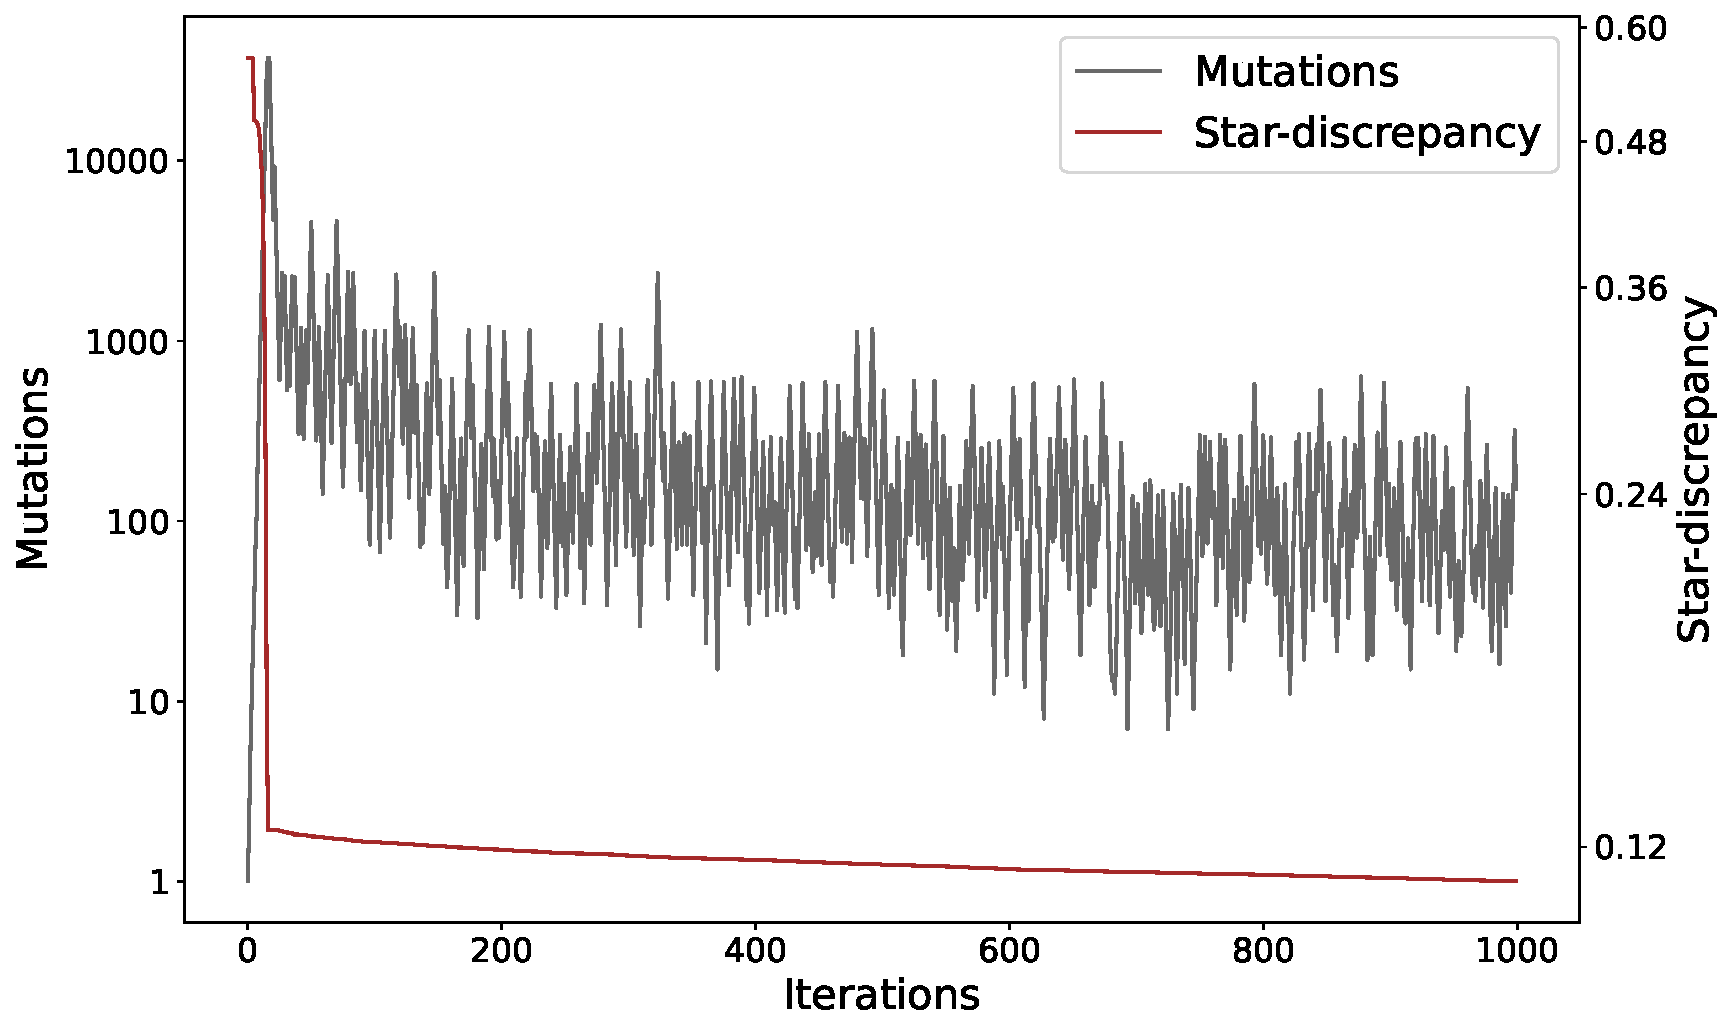
\includegraphics[width=\linewidth,trim=0 0 0 0,clip]{fig13.pdf}
\vspace{-7mm}
\caption{Evolution of the interaction graph: discrepancy (of user behaviour) and number of mutations performed. As the mutation rate only provides a probability of mutation, the actual number of the mutations typically differs from multiples of two.}
\label{fig:convergence}
\end{figure}

\section{Execution (Stage 3/3)}\label{sec:eval}

In this section, we present our approach for executing and evaluating community interaction. 

\subsection{Benchmarking the Evolutionary Approach}

A natural question is how to compare the Original and Evolved edge lists, because they are noteworthy different size? To compare the two, we craft additional datasets using two approaches. The first approach creates a larger version (called ``Simple'') of the original edge list by copying only the existing events until the size of this simple version matched that of the evolved edge list. The second approach generates new connections at random until the edge list reached the same size as the evolved one; the resulting community interaction is called ``Random''. In both approaches, we ensure that the number of FollowEvents is the same, as these events are considerably more numerous than other types of events. 
By reducing the potential impact of differences in size on the validity of the results, these approaches allow for the creation of comparable versions of the Original and Evolved interactions. 

\begin{table}
\centering
\caption{Dataset comparison, frequency of events}\vspace{-2mm}
\label{table:alldatasets}
\begin{tabular}{ccccc}
  \toprule
  \textbf{Event type} & \textbf{Original} & \textbf{Simple} & \textbf{Random} & \textbf{Evolved}\\
  \midrule
  FollowEvent & 195241 & 515841 & 515841 & 515841 \\
  PushEvent & 4234  & 11179 & 6943 & 6330\\
  WatchEvent & 1206  & 3163 & 3815 & 4123\\
  PullRequestEvent & 852  & 2186 & 3681 & 3718\\
  ForkEvent & 450  & 1174 & 3263 & 3531\\
  \midrule
  \textbf{Total} & \textbf{201983} & \textbf{533543} & \textbf{533543} & \textbf{533543} \\
  \bottomrule
\end{tabular}
\end{table}

\begin{figure}
\centering\vspace{-2mm}%
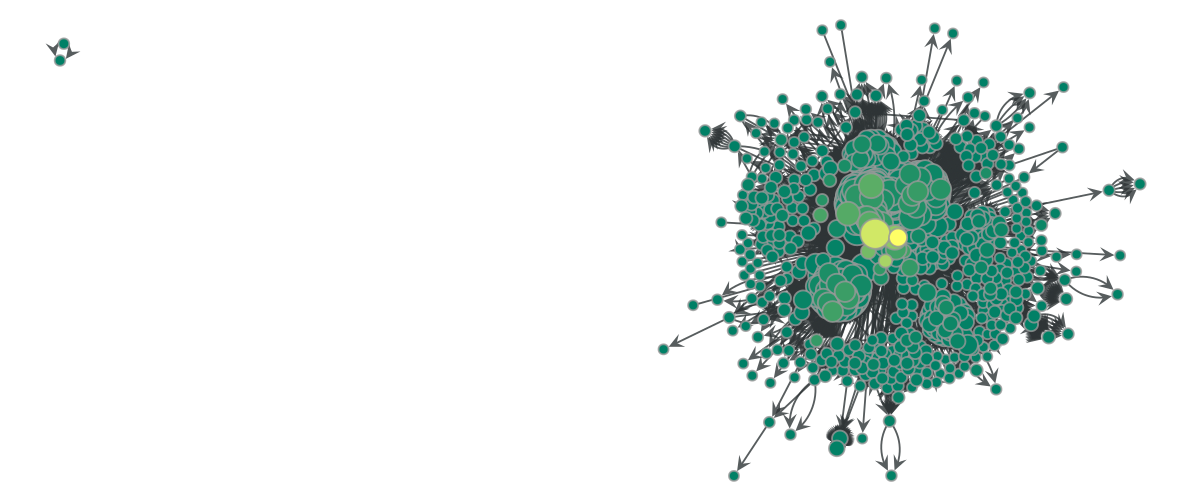
\includegraphics[width=0.41\linewidth,trim=650 0 0 0,clip]{Original_network_1k.png} 
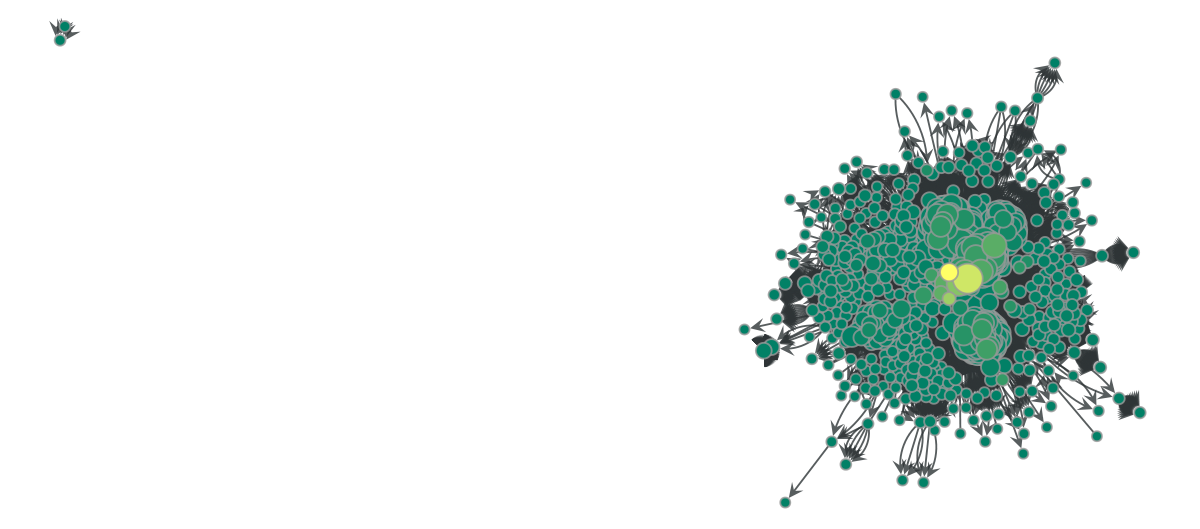
\includegraphics[width=0.395\linewidth,trim=720 0 0 20,clip]{Simple_network_1k.png}\\
(a) Original \hspace{20mm} (b) Simple \hspace{2mm}\;\\
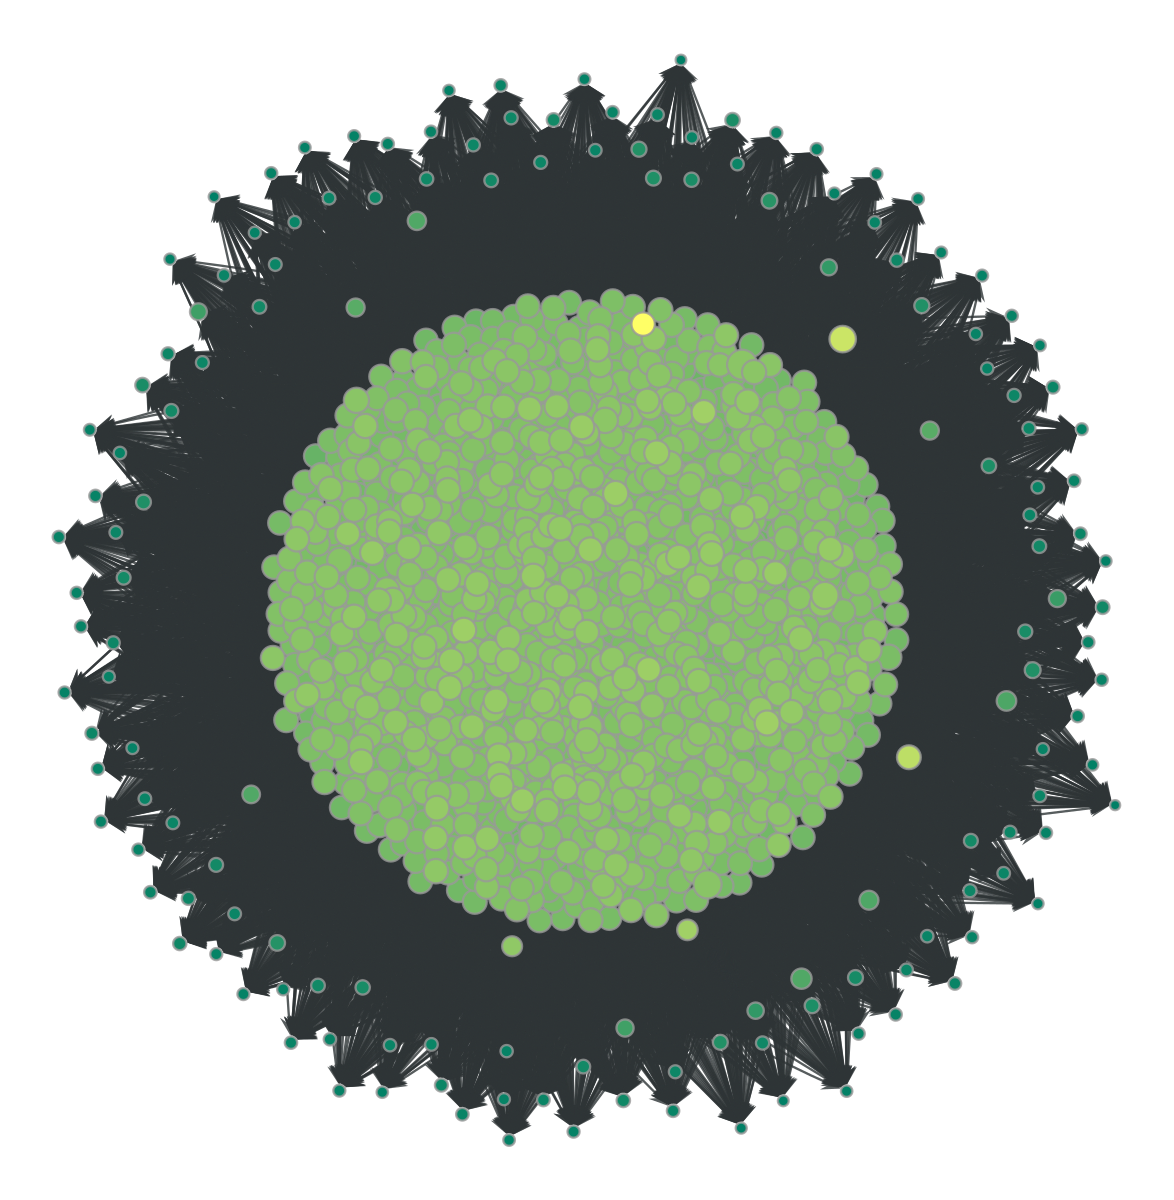
\includegraphics[width=0.385\linewidth,trim=0 0 0 0,clip]{Random_network_1k.png}
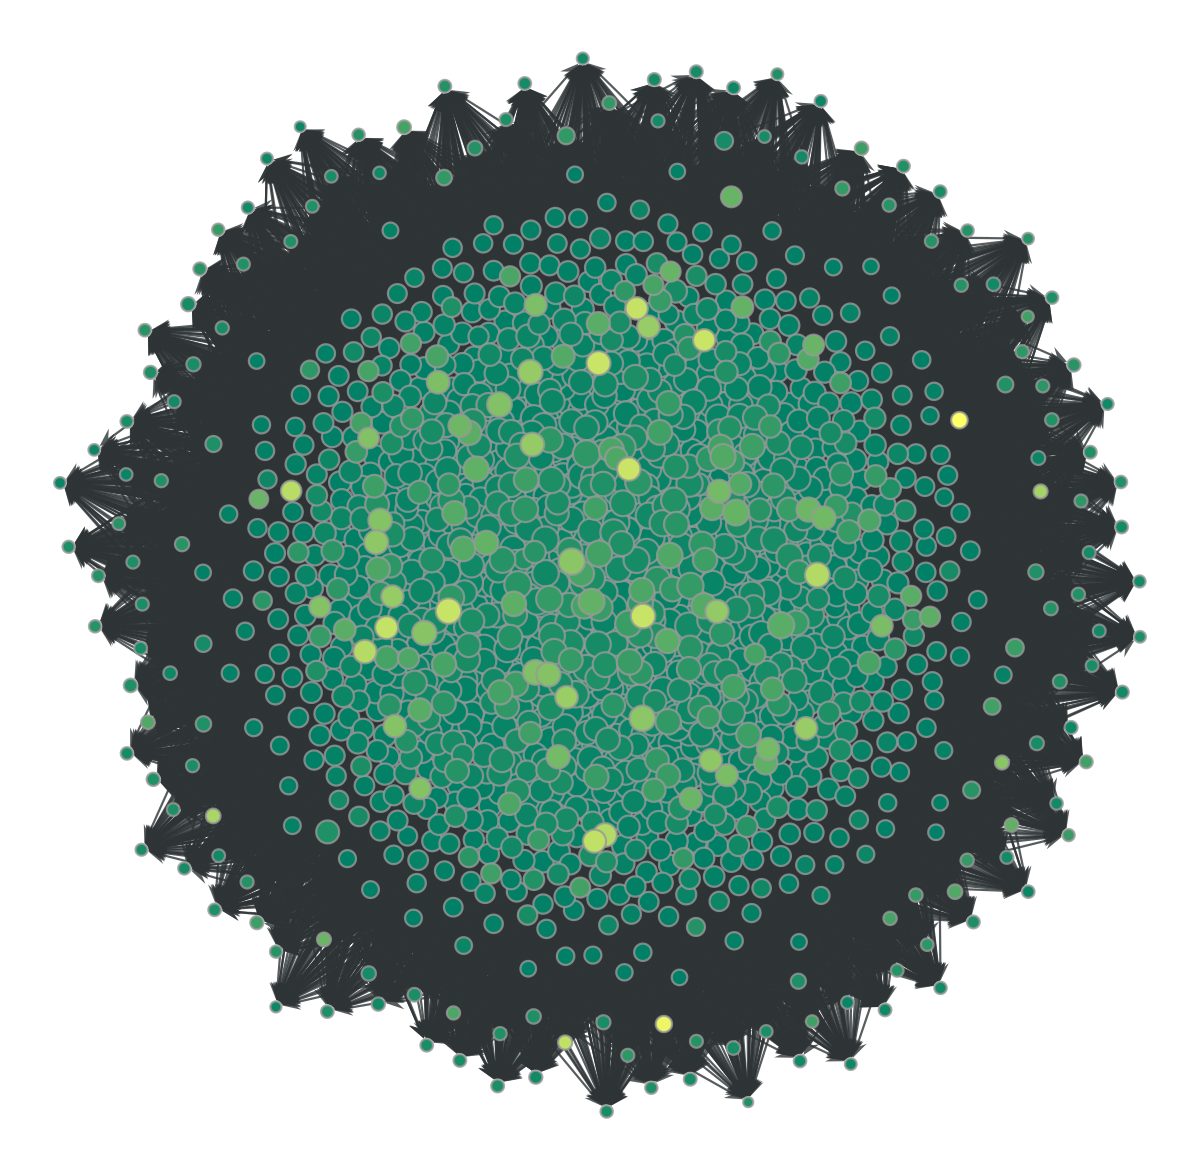
\includegraphics[width=0.4\linewidth,trim=0 0 0 0,clip]{Evolved_network_1k.png}\\
(c) Random \hspace{19mm} (d) Evolved
\vspace{-1mm}\caption{Projection of interaction graphs into 2d. The Original and Simple graphs each contain a connected component with only two users that is not shown here.}
\label{fig:projection}
\end{figure}

\begin{figure}
\centering

 \rotatebox{90}{\hspace{1mm} Evolved \qquad Random \qquad Simple \qquad Original}\:%\includegraphics[width=0.961\linewidth,trim=250 155 170 170,clip]{3Dplus2D_All.pdf}%
 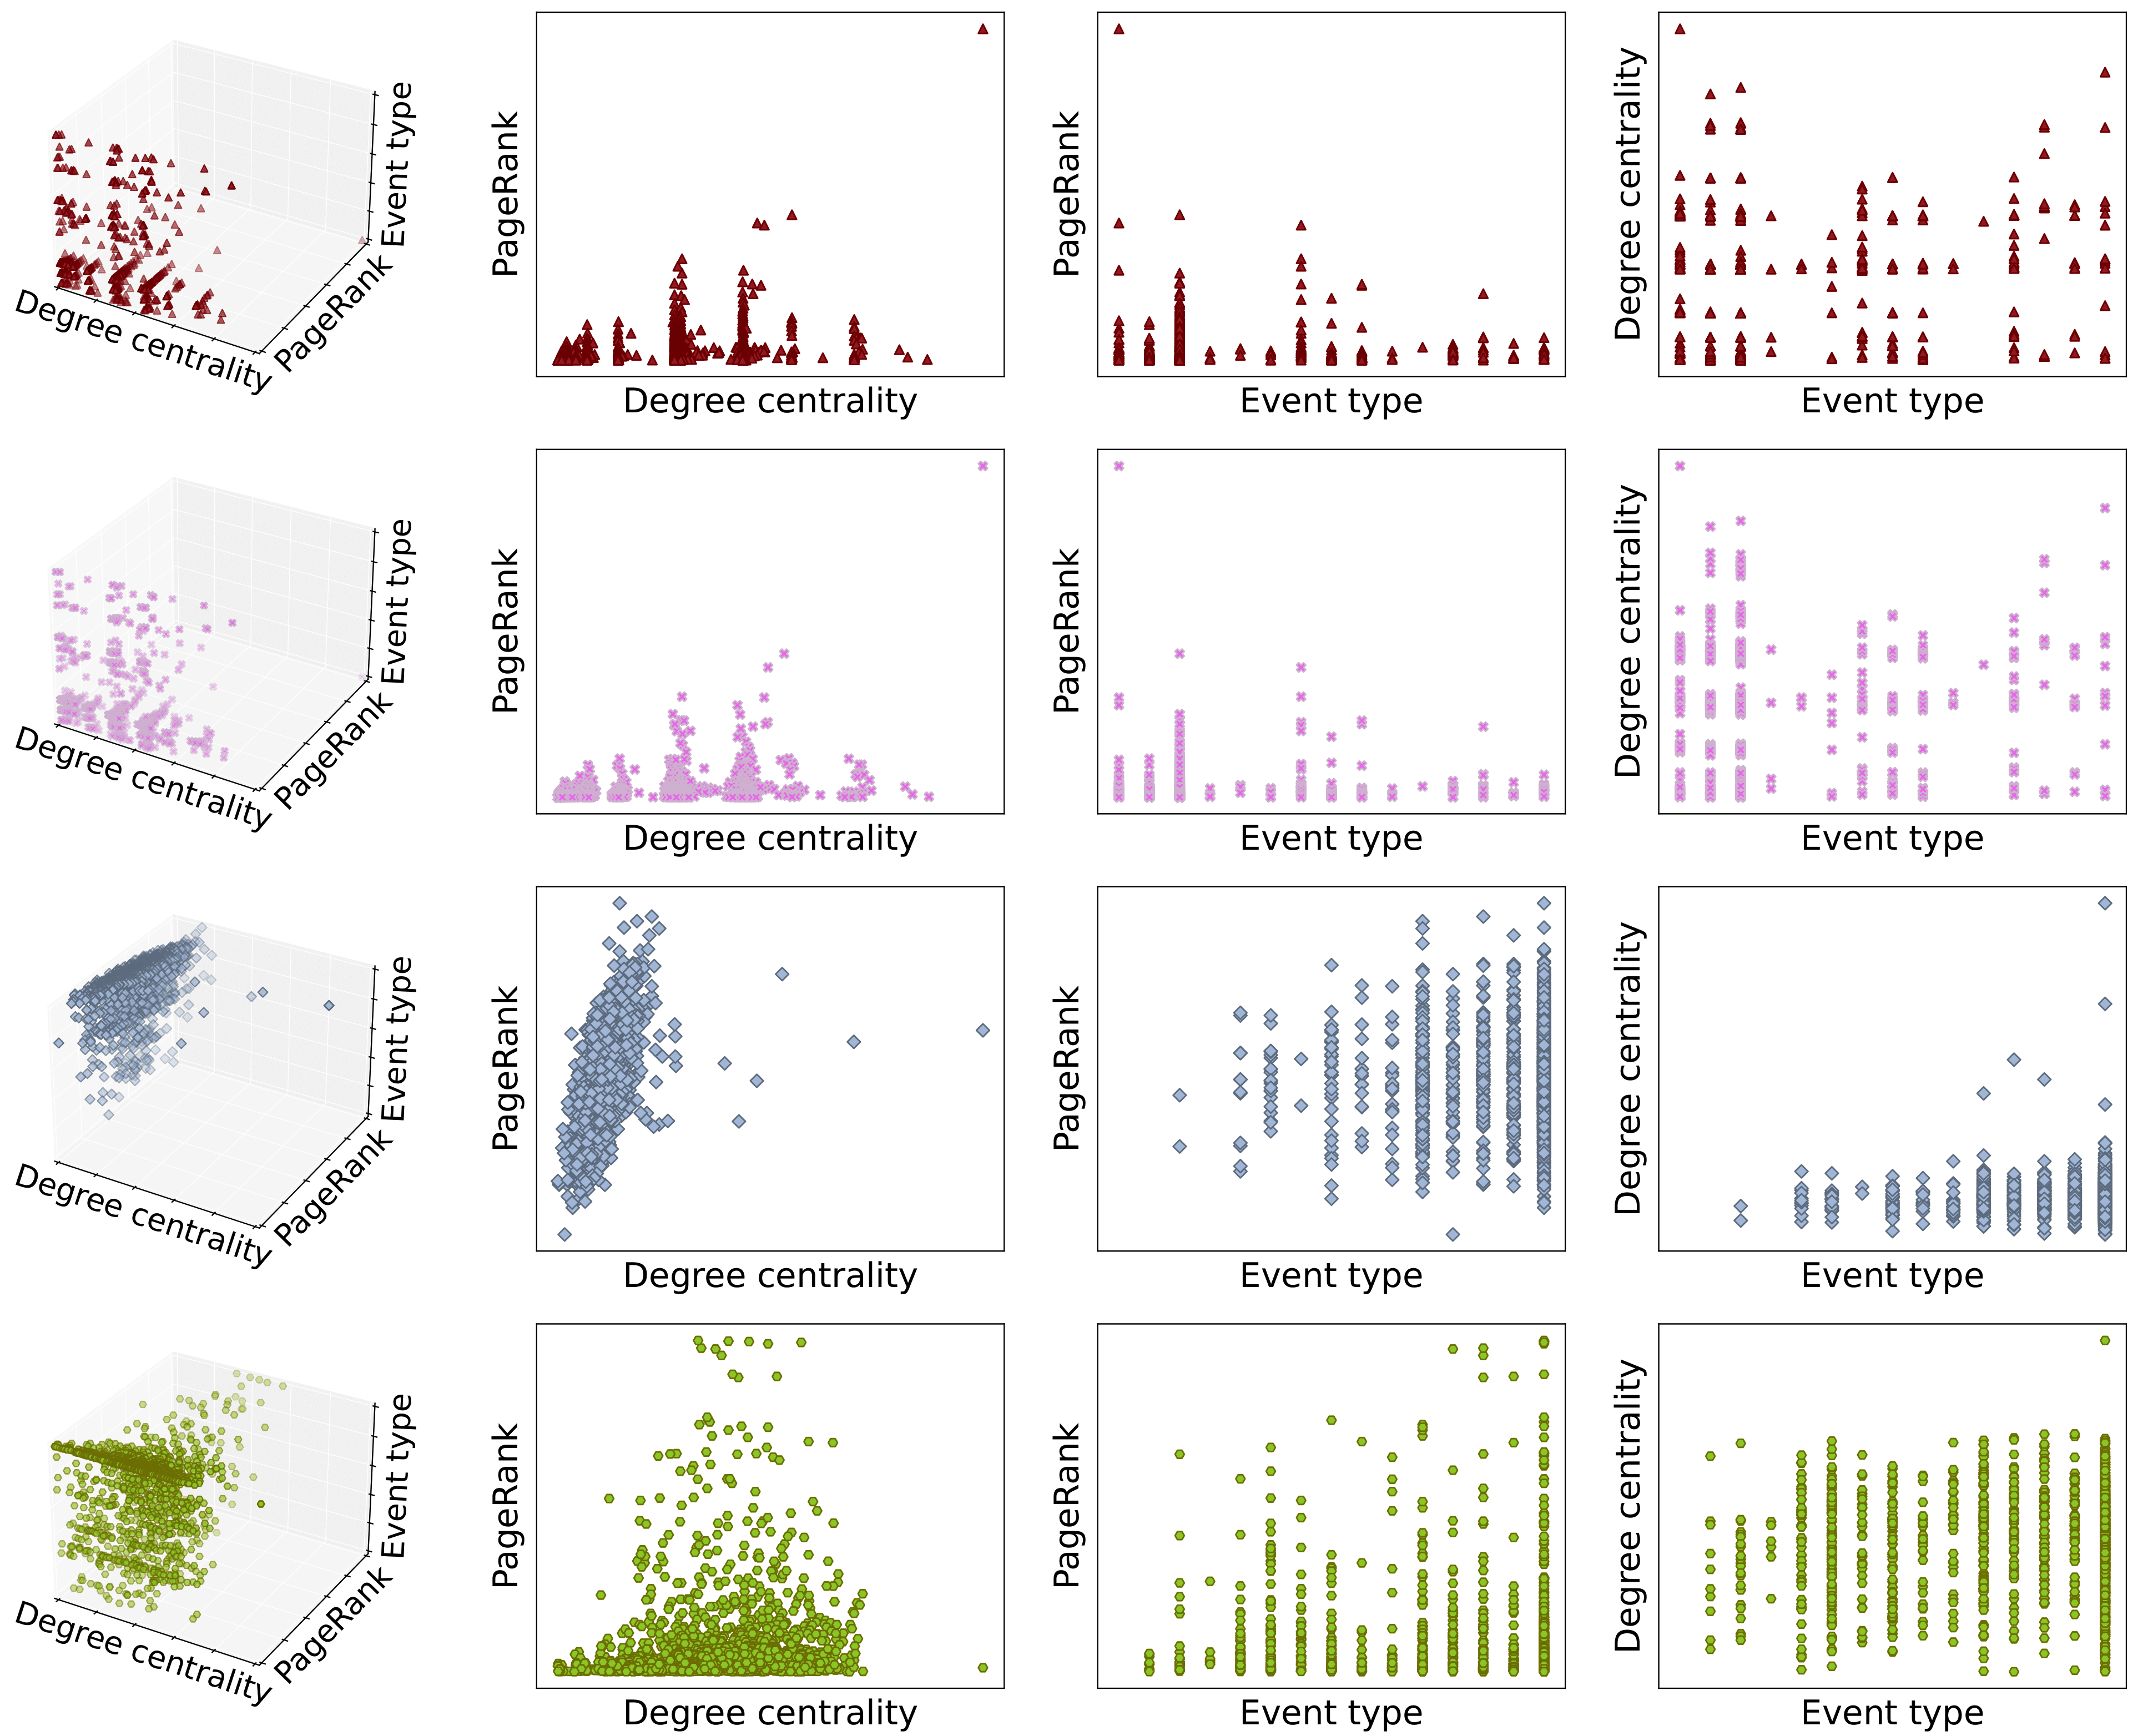
\includegraphics[width=0.961\linewidth,trim=0 0 0 0,clip]{3Dplus2D_All_v3.png}%
\vspace{-3mm}%
\caption{Dataset comparison: user interaction based on interaction features. The 2d plots are projections of the 3d plots in the leftmost column. The value ranges are always $\left[0,1\right]$.}
\label{fig:featurespace}
\end{figure}

Table~\ref{table:alldatasets} shows a first comparison between the four interaction graphs: the Original one that is directly based on GitHub data, its Simple (but larger) version, the Random version, and the Evolved one. 
Figures~\ref{fig:projection} and~\ref{fig:featurespace} add to this by presenting visualisations of the four communities. 
Figure~\ref{fig:projection} shows a projection of the graphs into 2d. Edges refer to interactions between users and repositories. 
Dot size represents the degree centrality of a node with larger dots indicating a higher degree centrality. 
In addition, the colour of each dot represents the PageRank score of the node, where the colour range from green, less important, to yellow, higher score.
As we can see, the Original and the Simple ones are (subjectively) close in structure, while the Evolved and the Random ones are also similar due to the high level of connectedness, but the Evolved one is much more diverse in terms of the distribution of PageRank scores and degree centrality. 

Figure~\ref{fig:featurespace} complements these observations by shoing the three features used to calculate the star-discrepancy score for each dataset, i.e. the degree of centrality of each user, their PageRank score, and the combination of events they are involved with. The visualisations show that users in the Original and Simple datasets tend to cluster together and occupy a smaller space, while users in the evolved edge list and the random version of the original edge list appear to be more evenly distributed throughout the space. Interestingly, even the random version achieves a fairly diverse set of interactions, although the degree centrality seems much less covered by the random dataset when compared to the evolved dataset. Overall, this data suggests that our evolutionary algorithm effectively improves the distribution of users in the feature space.

\subsection{Observing effects of community interactions}

To assess the impact that the different datasets have on the server, we consider the processing of the community interaction as an actual benchmark in itself: as the hundreds of thousands events are processed between the 1523 users on the server, we observe how the system behaves. 
In the following, we present the workflow used when executing the event and we present our observations.

\subsubsection{Methodology}

We require an elaborate workflow (see Figure~\ref{fig:image3}) as the randomised events create a broad range of situations that need to be dealt with; they would otherwise simply results in a myriad of errors. Essentially, all types of events are first validated by checking GitLab~CE's database to see if the user triggering the event exists. If not, the user is created. The same process is followed for the user and/or repository targeted in the event. The flow then proceeds to the corresponding action for that event.

\begin{figure*}
\centering\vspace{-4mm}
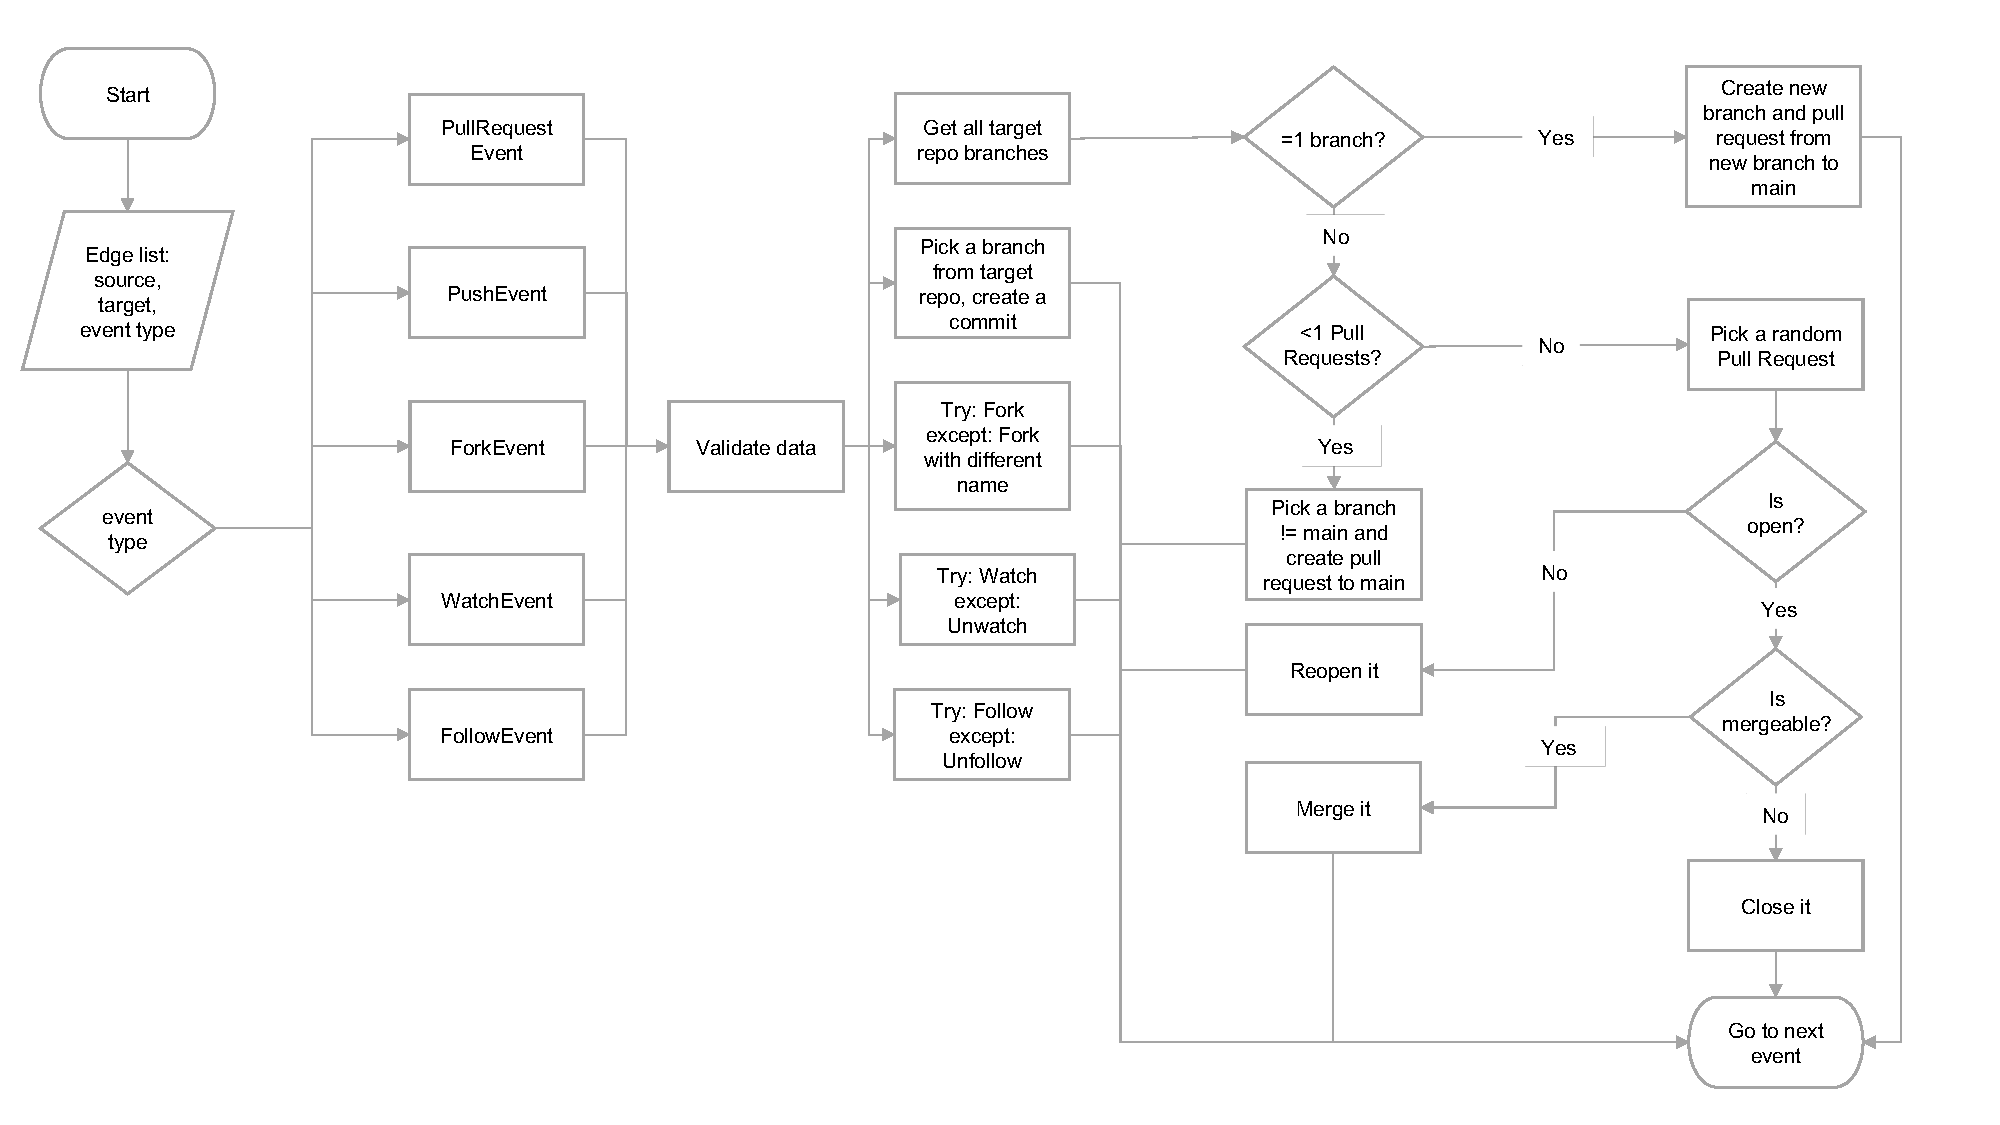
\includegraphics[width=\linewidth]{Flowchart.pdf}
\vspace{-13mm}
\caption{Workflow used when processing interaction graphs in GitLab.}
\label{fig:image3}
\end{figure*}

A complex logic is required for pull request events, where we select or create a branch to submit a pull request. If there is already an open pull request on that branch, we try to merge it. Otherwise, we close the event. If the pull request is closed, we reopen it. To add some realism, % and parallelism, 
we use a corpus of words that we extracted from the original dataset, so when we create a commit or a pull request, we add a random text from this corpus, allowing the system to check how many lines of text were added or deleted following Git logic.

On the technical side, we use the previously described setup with GitLab~CE and the virtual machine. 
Our GitLab API wrapper code implements the workflow and is used to load our datasets (Original, Evolved, Simple, and Random). 
During the processing, we collect performance data from the internal Grafana dashboard panels and from the Prometheus database (see Section~\ref{sec:methodology}) included in the GitLab installation. As substantial development effort has gone into developing the evaluation environment, we make the four Docker images publicly available at \url{https://github.com/fzanart/Socialz/}.

The processing of all community interactions is time-consuming: the execution of the Original/Evolved/Simple/Random datasets on four identical virtual machines takes 9.9/33.3/27.2/31.7 hours.

\subsubsection{Effects on the system}

\begin{figure}
\centering\vspace{-1mm}%

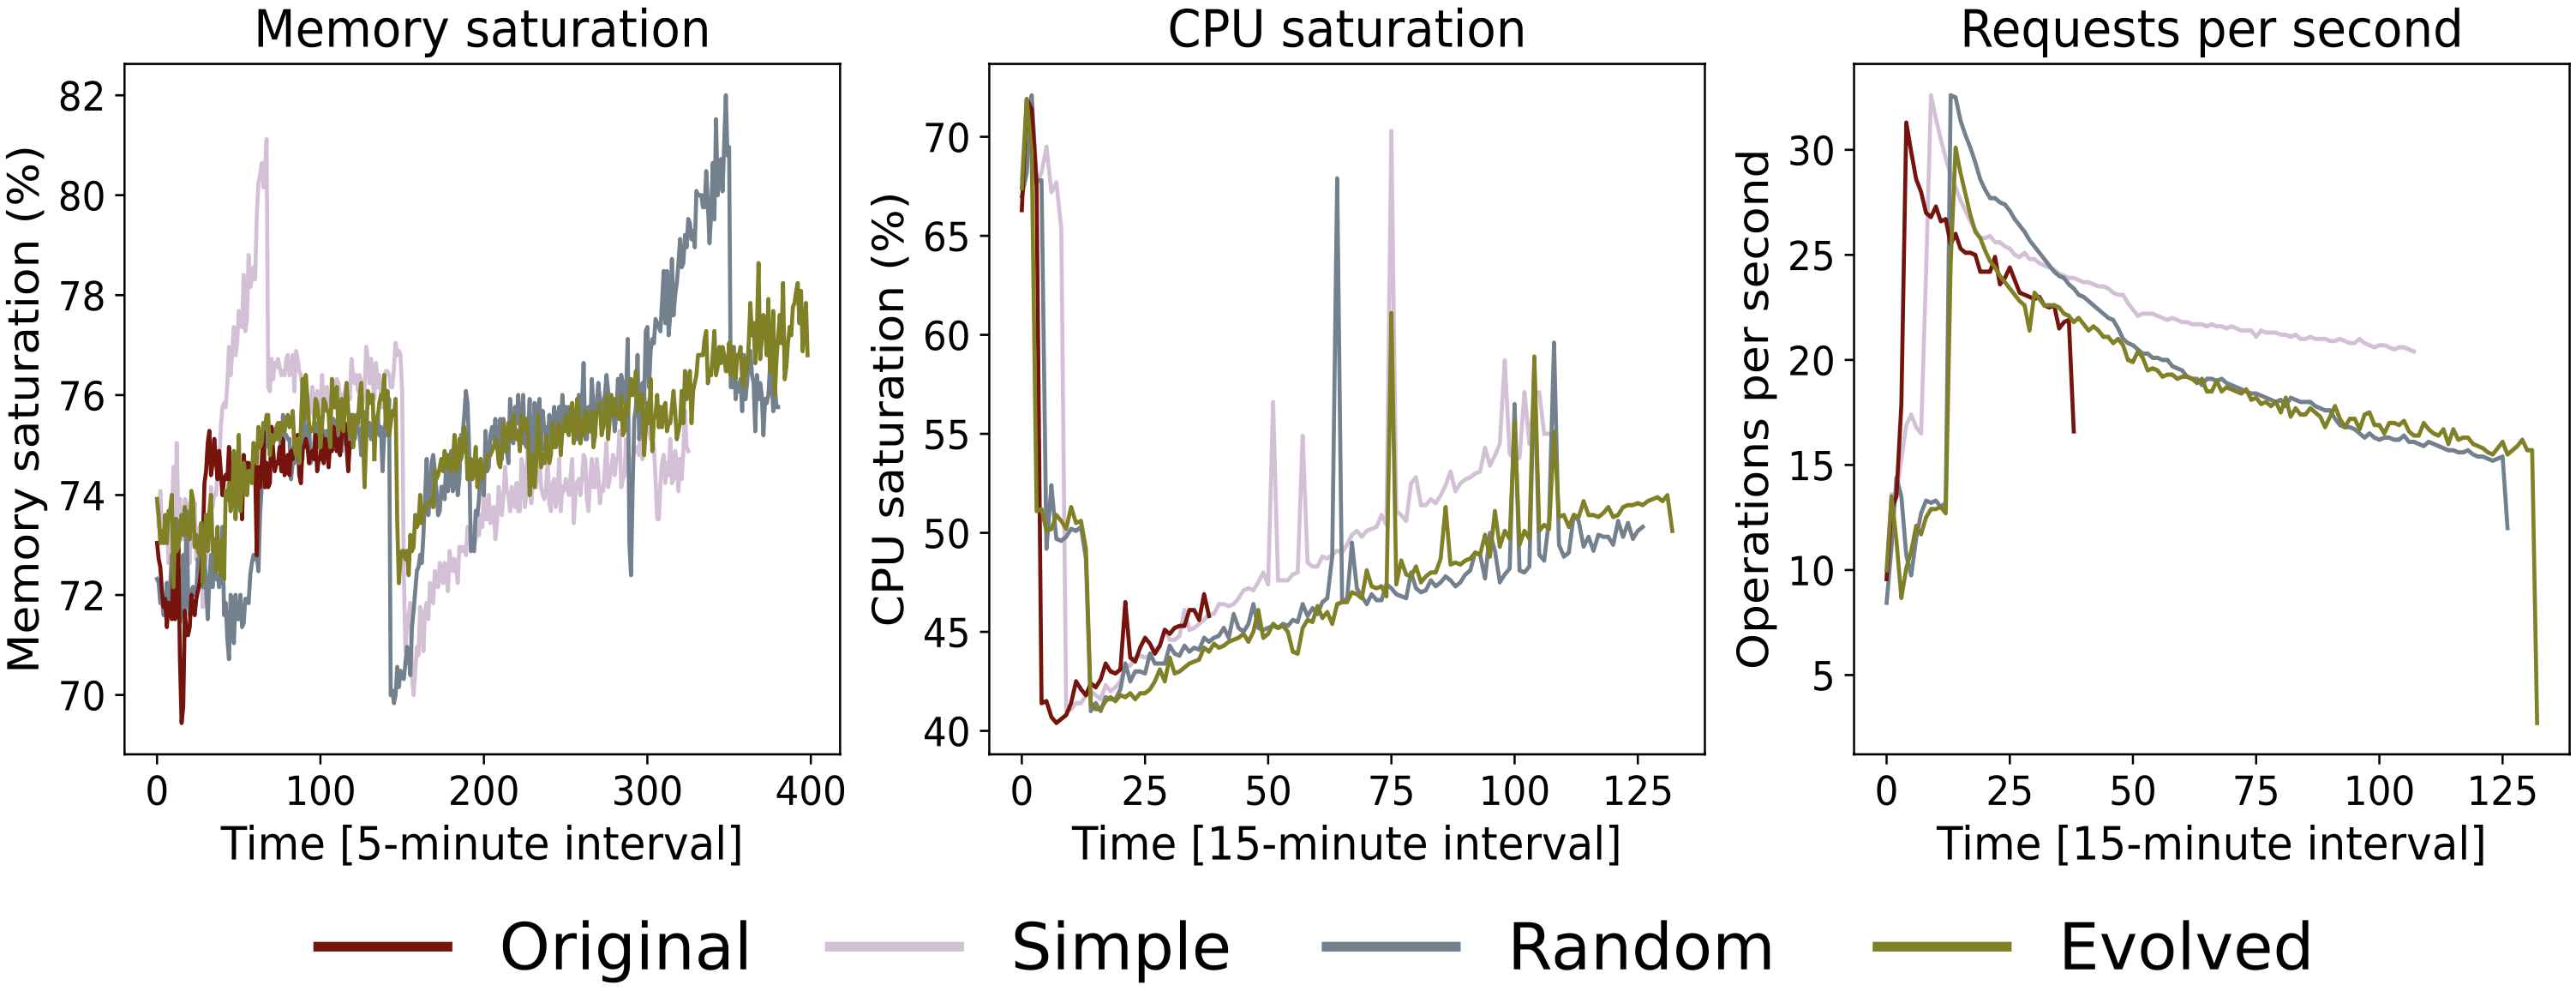
\includegraphics[height=33mm,width=\linewidth]{processingCommunityInteractionsOVERTIME.png}%
\vspace{-3mm}
\caption{Processing of community interactions. The sharp drops at the rightmost end of some data series are due to data aggregation used by the Prometheus database.}
\label{fig:prometheus}
\end{figure}

First, Figure~\ref{fig:prometheus} shows --- over time --- the memory utilisation, the CPU saturation, and the requests per second. 
As we can see, all four interaction graphs result in different workloads over time. 
We can make a few major observations. 
First, considering the memory consumption, the Evolved data set appears to result in fewer sharp increases than the other three; the same observation holds for the CPU saturation, where Simple and Random appear to have more and larger spikes than Evolved.
Second, while the Evolved and Random ones appear to affect the system in similar ways (with the respective data being very similar), the Simple one results in a higher CPU saturation while also being able to process more requests per second; this appears to be contradictory at first, and we can only conjecture that the Simple one exercises the system differently, possibly due to the higher proportion of PushEvents, but other explanations are possible, too.
Third, regarding the the major drop in memory consumption by 4--8\% at about 12 hours into the processing, we conjecture that this is due to a scheduled maintenance; interestingly, this drop does not seem to have obvious effects on the CPU saturation or on the number of processed requests per second. 

\begin{figure}
\centering%
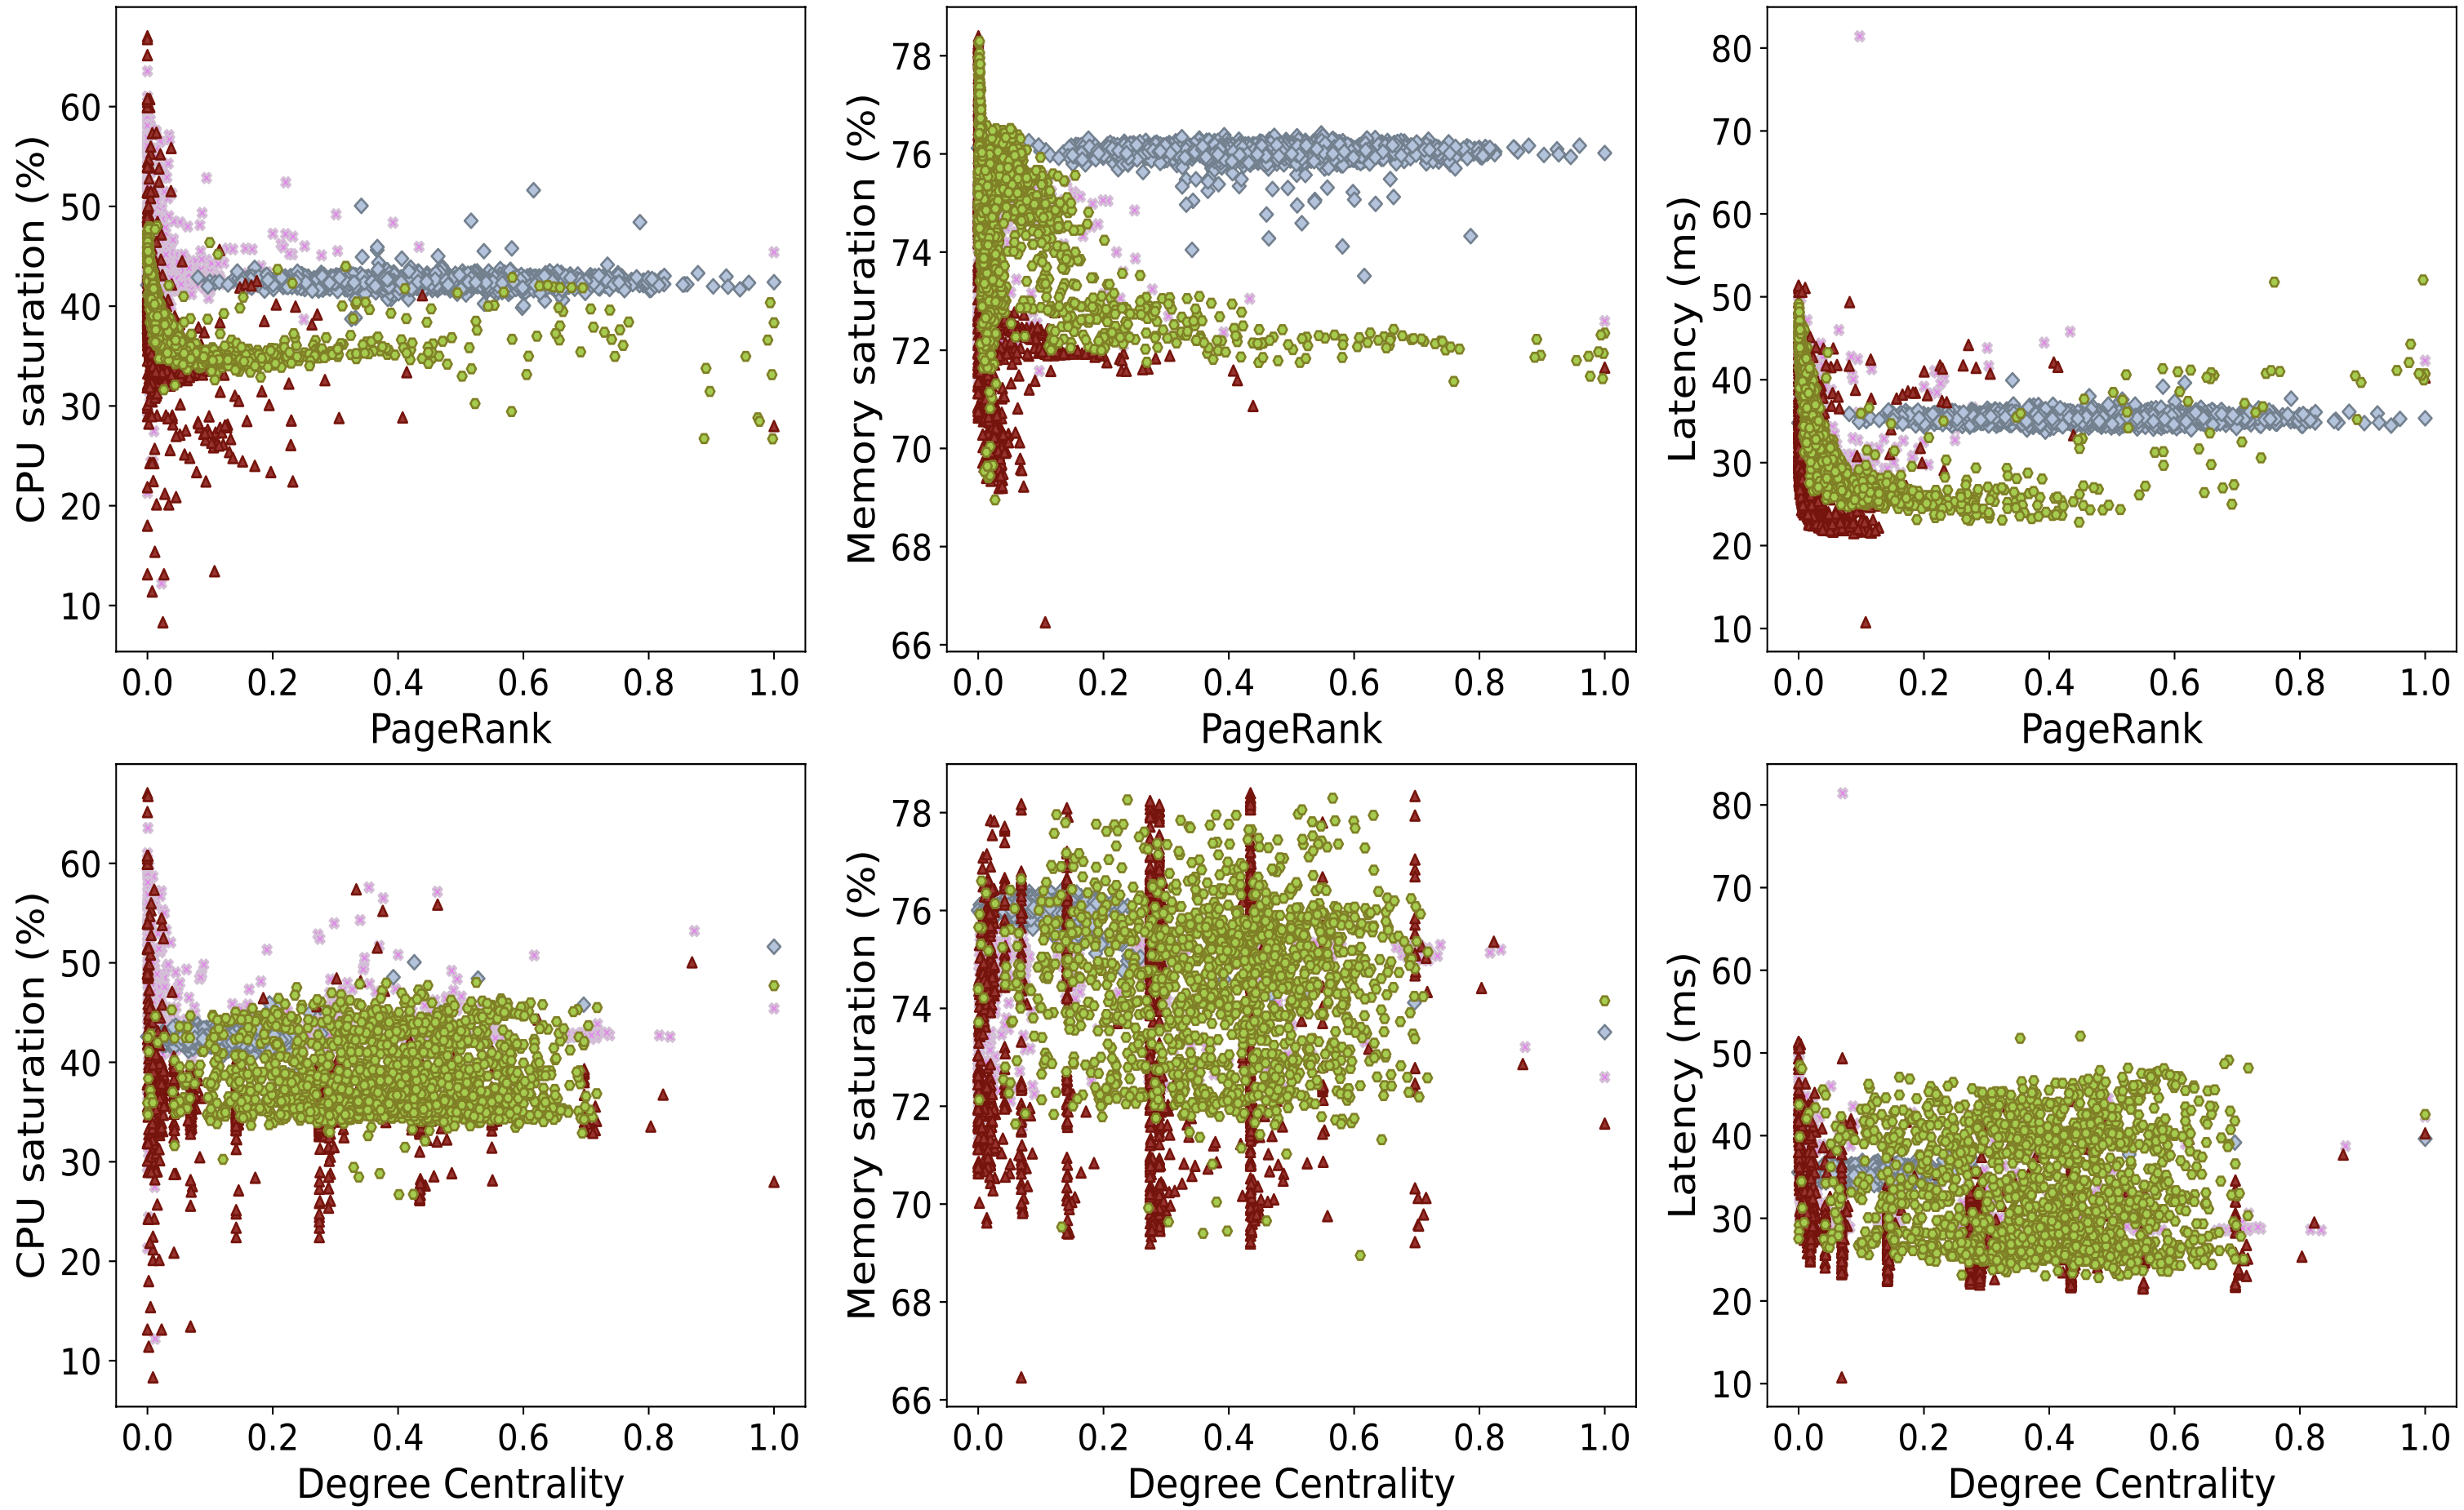
\includegraphics[width=\linewidth,trim=0 0 0 0,clip]{corr1.png}\\
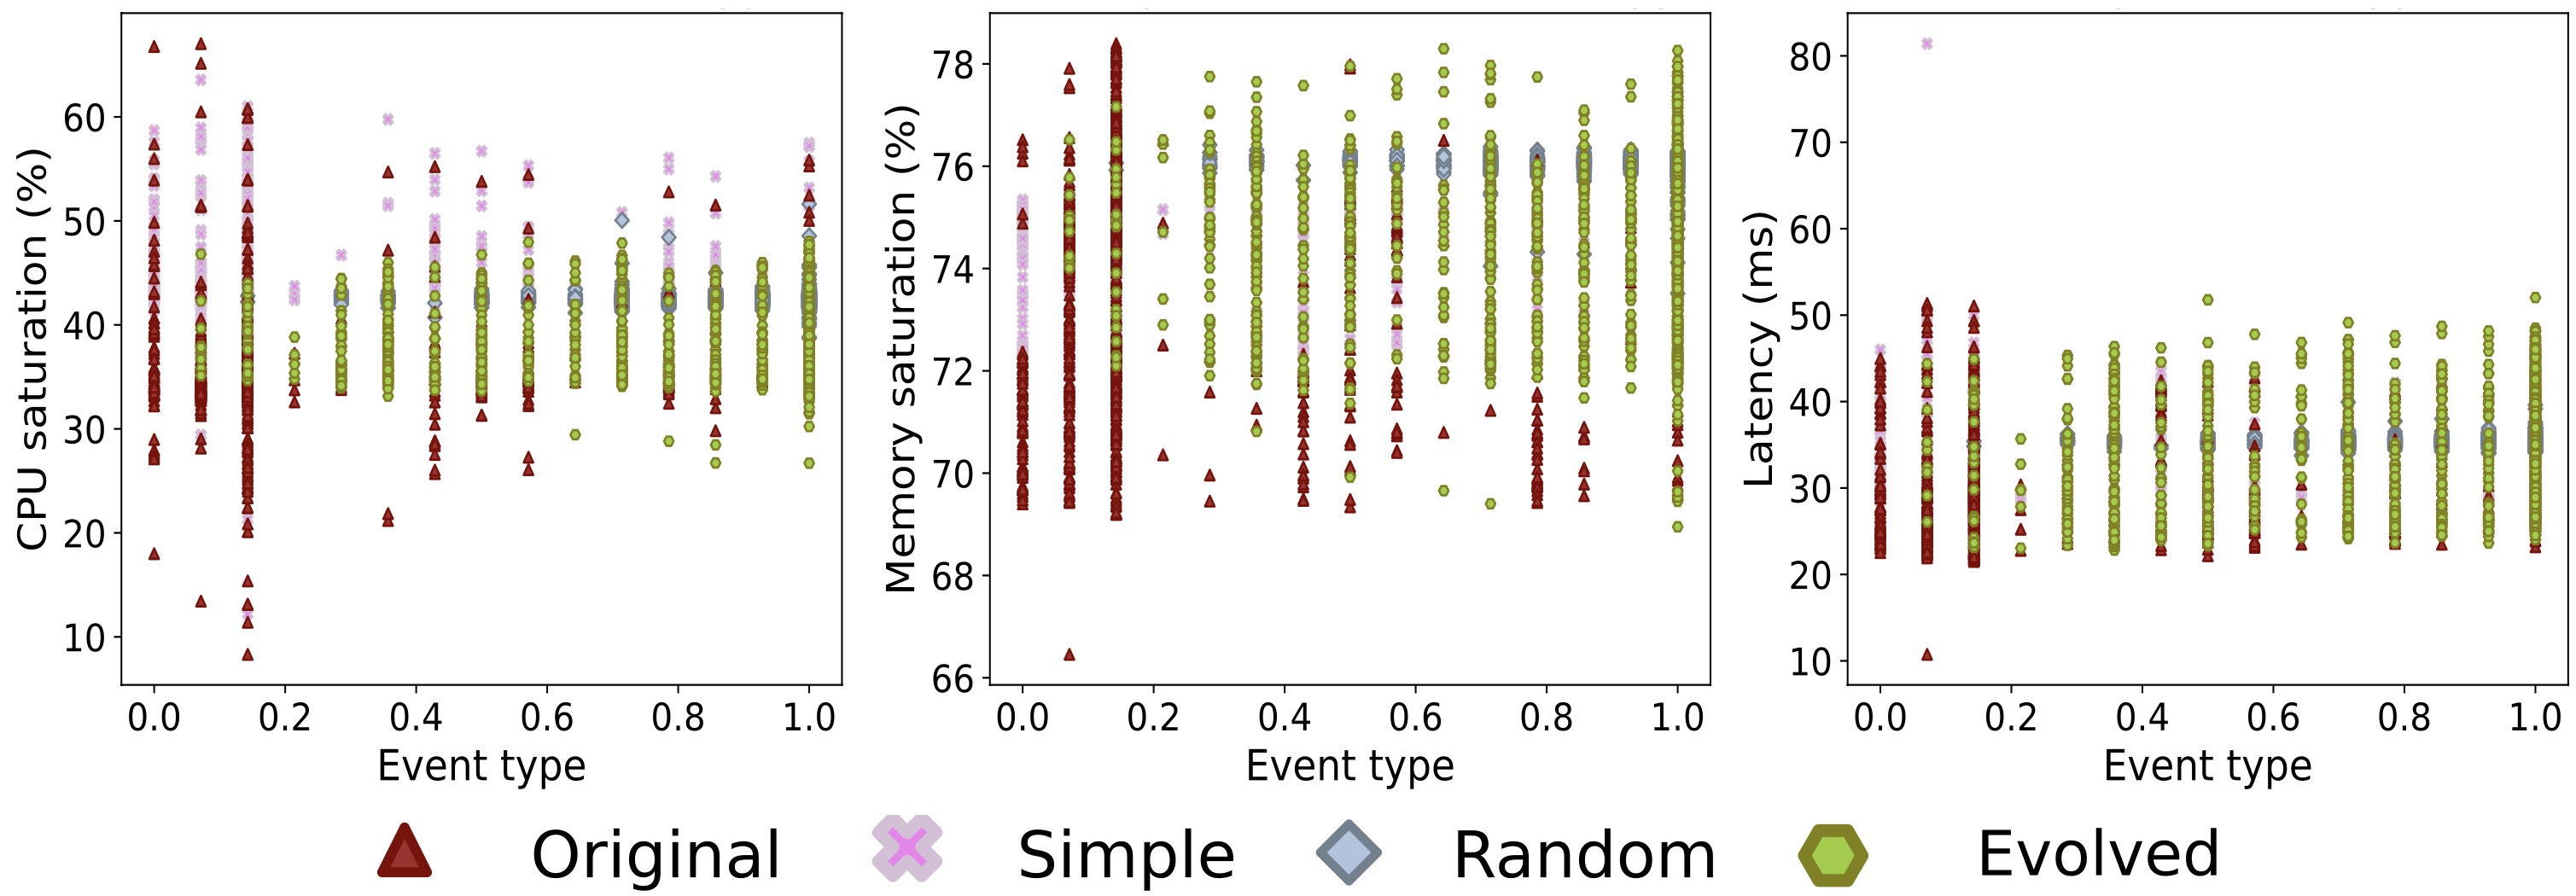
\includegraphics[width=\linewidth,trim=0 0 0 0,clip]{corr2.png}
\vspace{-5mm}
\caption{Correlation of user features and resource utilisation. Shown are the averages for each of the 1523 users.}
\label{fig:correlation}\vspace{-2mm}
\end{figure}

In order to gain further insight into user behaviour and its impact on the system, we present a correlation analysis in Figure~\ref{fig:correlation} between three feature metrics (PageRank, Degree centrality, and Event types) and three resource utilization metrics (CPU saturation, Memory saturation, and Latency), averaging results for each user. Despite acknowledging the fluctuation in performance over time as illustrated in Figure~\ref{fig:prometheus}, our analysis identifies several statistically significant differences.
For instance, while all three community interactions involve changes to the original dataset, our findings demonstrate that sometimes these evolved interactions impact the server in a manner that is more similar to the original dataset rather than simple or random modifications.

Specifically, we observe strong negative Spearman correlations (coefficients $-0.69 \leq r \leq -0.62 $, $p<1\%$) between PageRank and CPU, Memory, and Latency in the original data, which is maintained in the evolved dataset. Conversely, no correlation ($|r|<0.1$) is observed in effects of Simple and Random. This observation leads us to hypothesise that a high number of connections between irrelevant users may increase system load, as the system has to execute expensive tasks such as creating these users and connections. On the other hand, relevant users with many connections have already executed several tasks that do not need to be repeated, such as creating new repositories, which could reduce system load.

With regards to degree centrality, while we can make out visual differences in the data, we do not observe any outstanding relationships when considering Spearman correlation; we do only observe similar ranges of CPU and Memory utilisation and Latency between the original, simple, and evolved datasets. The random dataset occupy a smaller range, while the evolved dataset looks more spread out due to optimisation. Finally, the data on the event types overlaps much due to the discrete nature of the event types; the correlations are weak (if at all) at $|r|<0.2$. 

\subsubsection{Characterisation of the Performance Indicators}

In our first attempt to evaluate the potential usefulness of performance indicators during the evolution of community interaction in-vivo on a server, we have identified three main observations. 

First, we have noticed that neighboring data points in Figure~\ref{fig:prometheus} often show variation due to what seems to be random noise, making it challenging to compare marginal differences that may be impacted by factors outside of our control. In addition, we can see from Figure~\ref{fig:correlation} that users who are similar, such as having the same PageRank or degree centrality, can still have different experiences in terms of server load, making it potentially difficult to develop a surrogate model.

Second, we have observed that disruptive events can be triggered by processes running on the virtual machine or by GitLab CE's own management, which can have a significant impact on the performance of the server.

Third, we have noted significant changes in the performance of the server at the start of the evaluation, where there is a sudden change observed after just a few minutes or hours. These changes may be indicative of major state changes that occur during the evolution of community interaction on the server.

\subsubsection{Found limitation}

Our case study has uncovered a crucial issue with the server that could not have been detected through a simple repetition of the Simple dataset. During our investigations, we found that GitLab imposes limits to ensure optimal performance quality. In particular, our initial experiments revealed a restriction on the maximum number of followed users to 300. This was confirmed by a review of public issue comments in GitLab, which indicated that this limit was in place to prevent the activity page for followed users from failing to load~\cite{Issue360755}. In our case,  tests resulted in HTTP 304 errors when trying to load follow events for users who were following more than 300 users, causing the event creation to fail. 
To resolve this issue, we manually edited GitLab's source code to increase the limit to 1,523, the total number of users in our dataset. 
It is important to mention that for our use case, we do not access the activity page for followed users, so we conjecture that our modification of the source code does not have any adverse impact on our results. Hence, we see this as a good illustration of how diverse data can outperform original data for testing configurations: a broader range of data points offers more chances of uncovering issues, making it a valuable asset for any testing process.

\section{Efficient evolution and evaluation}

In conclusion of this first case study of Socialz, we would like to bring attention to two important research questions: how can we efficiently evolve and evaluate community interaction?

Efficiently evolving community interaction is crucial as it allows for iterative improvements and explorations based on observed data, increasing the chances of identifying social bugs. 
It may be beneficial to evolve interactions either 
(1) in-vivo, i.e. small-scale interactions are evaluated ``live'' on a running server, or 
(2) to run comprehensive evaluations for each large community interaction akin to those performed in Section~\ref{sec:eval}. 
However, small-scale evaluations come with the challenge of affecting the virtual machine and creating unintended side-effects, such as triggering memory clean-ups or altering the system's performance over time, as seen in Figure~\ref{fig:prometheus}. 
In contrast to this, comprehensive analyses of the entire community interaction (which may involve hundreds of thousands of events like in our case) are time-consuming, taking over one day each. 
As a middle way between these two extremes, differential evaluations may be a solution, but only if the effects of mutations can be attributed efficiently and accurately. Currently, this presents a significant challenge both in practice and algorithmically.

The question of how much to evolve community interaction is closely tied to the question of which performance indicators should be used. As our data analysis has shown, there is a significant amount of noise present in the server under examination. This is a common issue in complex systems such as Android phones~\cite{bokhari2020validation}, where the targeted application shares resources with multiple processes and modern multi-core hardware. Existing validation methods, such as complete rollbacks to known states or extended repetition, are not practical due to the time and resources required. Therefore, there is a need for schemes that allow for reliable and efficient attribution of community interactions to their effects.

\section{Conclusions and Future Work}

This study presents a new social fuzz testing method called Socialz, which is based on publicly accessible data from GitHub. The approach uses evolutionary computation to diversify community interactions, and then evaluates the results on a GitLab~CE server.

The key takeaways of this research are: 
\begin{itemize}
    \item Social fuzz testing is a feasible approach, although the initial setup requires significant effort. 
    \item Evolutionary diversity optimisation can generate community interactions that are significantly different from the original data or random data, potentially uncovering social bugs. 
    \item Our testing also revealed a limitation that simple data replay could not.
\end{itemize}

In addition to the already outlined research directions on efficient evolution and evaluation, future work in this area offers endless possibilities, such as: 
\begin{itemize}
    \item Further characterisation and hybridisation of sub-communities.
    \item Exploration of additional community interactions and the related features.
    \item Integration of Socialz with traditional fuzz testing techniques that target code-level or system-level interactions.
\end{itemize}

To support future research in social testing, the code, data, and virtual machines used in this study are available for public use at  \url{https://github.com/fzanart/Socialz/}.

\subsection*{Acknowledgements}

This project has been enabled by a gift from Facebook/Meta: \url{https://research.facebook.com/blog/2021/9/announcing-the-winners-of-the-2021-rfp-on-agent-based-user-interaction-simulation-to-find-and-fix-integrity-and-privacy-issues/}

\bibliographystyle{ACM-Reference-Format}
\bibliography{sample-base}
\end{document}
\endinput
